\documentclass{article}

\usepackage[spanish]{babel}
\usepackage[numbers,sort&compress]{natbib}
\usepackage[T1]{fontenc}
\usepackage[ansinew]{inputenc}
\usepackage{graphicx}
\usepackage{url}
\usepackage{subcaption}
\usepackage{caption}
\usepackage{float}
\usepackage{listings}
\usepackage{amsmath}
\usepackage[numbers,sort&compress]{natbib}

\begin{document}
\title{\textbf{Sistema Multiagente}}
\author{Anahi Elizabeth Llano Guerrero}

\maketitle

\section{Objetivo}\label{obj}

El objetivo \cite{elisa} consiste en vacunar con probabilidad $Pv$ a los agentes al momento de crearlos de tal forma que est\'an desde el inicio en el estado R y ya no podr\'an contagiarse ni propagar la infecci\'on. Estudiar el efecto estad\'istico del valor de $Pv$  (de cero a uno en pasos de 0.1) el porcentaje m\'aximo de infectados durante la simulaci\'on y el momento en el cual se alcanza ese m\'aximo.

\section{Metodolog\'{i}a}\label{met}

Para el an\'alisis, se realiz\'o una modificaci\'on del c\'odigo \citet{elisa} mostrado en clase de tal forma que se pudiera vacunar un porcentaje de los agentes desde el principio.


\begin{lstlisting}[language=R]
l <- 1.5     
n <- 50       #numero de agentes
pi <- 0.05  #probabilidad de infeccion al inicio
pr <- 0.02  #probabilidad de recuperacion
v <- l / 30 #velocidad del agente
r <- 0.1 
tmax <- 100 
PV <- seq(0,1,0.1)  #Probabilidad de la  vacunaal inicio  con las variaciones
datos <- data.frame()
for(pv in PV){   
  for(rep in 1:25){  #con 25 replicas
agentes <- data.frame(x = double(), y = double(),
                      dx = double(), dy = double(),
                      estado  = character())
for (i in 1:n) {                                                       
      if(runif(1) < pv){    #vacunados al inicio con probabilidad de pv
        e <- "R"
      } else if(runif(1) < pi){
        e <- "I"
      } else{
        e <- "S"
      }
\end{lstlisting}
  

El resto del c\'odigo \citep{ana} fue similar al mostrado en clase, de igual manera lo importante fue cumplir con el objetivo al agregarle una vacuna desde un principio, vacunar una cierta parte de los agentes, y as\'i mismo estudiarlo en pasos de 0 a 1 con pasos de 0.1, los resultados obtenidos fueron guardados y graficados en un diagrama de caja-bigote para un mejor an\'alisis.

\section{Resultados y Discusi\'{o}n}\label{res}


\begin{figure}[H]
       \begin{center}
           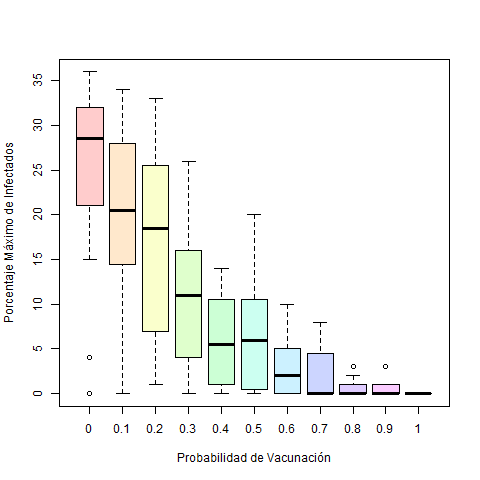
\includegraphics[width=13cm]{pr6sim.png}
       \end{center}
\caption{Porcentaje m\'aximo de infectados por variaci\'on de probabilidad}
        \label{f1}
\end{figure}
 
En la figura \ref{f1} se muestran los porcentajes m\'aximos de infectados en cada de las variaciones, se pude observar que conforme se van aumentando las probabilidades de vacunaci\'on inicial, disminuye la cantidad m\'axima de infectados, por lo cual se puede decir efectivamente la probabilidad de vacunaci\'on inicial tiene un efecto directo sobre el numero m\'aximo de infectados en la simulaci\'on.

\begin{figure}[H]
       \begin{center}
           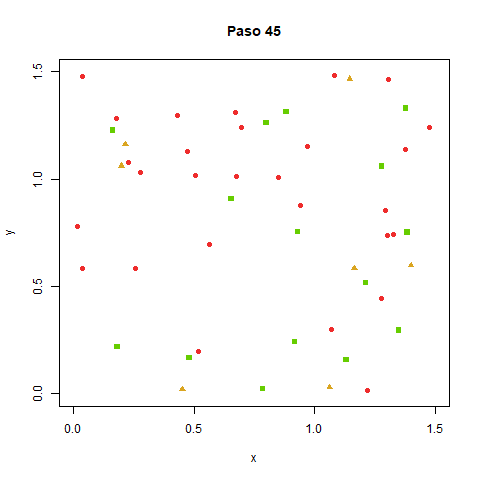
\includegraphics[width=13cm]{p6_t_t.png}
\end{center}
\caption{Iteraci\'on m\'axima en infectados}
        \label{f2}
\end{figure}
 
En la figura \ref{f2} se observa un sistema multiagente en donde tenemos m\'as infectados seg\'un los datos obtenidos se podr\'ia concluir que el mayor n\'umero de contagios normalmente se encuentra en iteraciones medias, es decir si tenemos un m\'aximo de 100 iteraciones el mayor n\'umero de contagios esta aproximadamente a la mitad de estas iteraciones.

\begin{table}[H]
 \centering
\caption{Maximos infectados por probabilidad}
\begin{tabular}{rrrr}
  \hline
 Probabilidad & M\'aximo & Porcentaje \\ 
  \hline
0 & 40 & 80 \\ 
 0.1 &30  & 60 \\ 
 0.2 & 33&66  \\ 
 0.3 & 24& 48 \\ 
 0.4 &19 & 38\\ 
 0.5 &  17& 34 \\ 
 0.6 & 8 &16 \\ 
 0.7 &  5&12 \\
 0.8 & 7 &14 \\
 0.9 &4  & 8 \\
 1 & 0& 0\\
   \hline
\end{tabular}
\label{t1}
\end{table}

 En el cuadro \ref{t1} se observa el porcentaje m\'aximo de infectados por probabilidad en donde se determina que donde hubo mayor caso de infectados fue cuando tenemos una probabilidad de 0, el n\'umero de infectados va disminuyendo conforme se va aumentando la probabilidad de vacunaci\'on , disminuimos de tener un 40 infectados a tener 0, aumentando esta probabilidad de vacunaci\'on.
se observan tambi\'en diferencias entre las probabilidades de vacunaci\'on y para  estas diferencias se realiz\'o un analisis estad\'istico ANOVA \citep{clara} para determinar si es que son significativas estas diferencias

\begin{table}[H]
 \caption{Comparaci\'on de los porcentajes del m\'aximo de agentes infectados con respecto a la probabilidad de vacunaci\'on}
 \begin{center}
 \begin{tabular}{r|r|r|r|r|r}
\texttt{} & \texttt{GL} & \texttt{Suma Cuad.} &\texttt{Media Cuad.} & \texttt{F}  & \texttt{Pr(>F)} \\
\hline
datos-probabilidad & 1 & 51169 & 51169 & 242.9 & <2e-16\\ 
\hline
Residuales & 218& 45927 & 211 \\ 
\end{tabular}
\end{center}
\label{t2}
\end{table}

En el cuadro \ref{t2} se observa el an\'alisis estad\'istico realizado en donde podemos afirmar que existen diferencias significativas en el n\'umero m\'aximo de infectados al variar la probabilidad de vacunaci\'on en una simulaci\'on de sistema multiagente.


\section{Conclusi\'{o}n}\label{con}
Al aumentar  la probabilidad de vacunaci\'on disminuye el porcentaje del n\'umero m\'aximo de infectados en una simulaci\'on de sistema multiagente.

\section{Reto 1}\label{ret}

Para el primer reto se cabio el patr\'on de movimiento a que no tenga una trayectoria fija, donde cada agente tiene una posici\'on meta $(x,y)$ hacia la cual se mueven con una velocidad $v$ al alcanzar (o superar) su meta, elige al azar una nueva meta uniformemente al azar. La velocidad de cada agente es una constante, normalmente distribuido sobre la poblaci\'on de agentes. 
Para esto, se mantienen las variaciones en la probabilidad de generar vacunados y el n\'umero de replicas.
Se declararon los puntos iniciales en los que aparecen los agentes y sus puntos meta, a su vez se genera un numero aleatorio de pasos con el que se calcula la velocidad con la que avanza el punto meta cada agente.

\begin{lstlisting}[language=R]
pasos <- sample(5:50,1) #Numero de pasos por recorrer
      xc <- runif(1,0,l) #Punto inicial en X
      yc <- runif(1,0,l) #Punto inicial en Y
      px = runif(1,0,l) #Punto meta en X
      py = runif(1,0,l) #Punto meta en Y
 \end{lstlisting}

Esto se genera dentro de un rango cero a el tama\~no del \'area en el que se mueven los agentes. para que la velocidad con la que llega al punto meta concuerde con la distancia en pasos que se recorre se realiza la siguiente operaci\'on.

\begin{lstlisting}[language=R]
vx = ((px - xc)/pasos) #Velocidad a la meta en X
      vy = ((py - yc)/pasos) #Velocidad a la meta en Y
\end{lstlisting}

De igual manera el resto del c\'odigo se modific\'o de tal manera de poder calcular el objetivo en el reto 1, as\'i mismo se guardaron los datos y graficaron en un diagrama de caja-bigote para su an\'alisis.

\begin{figure}[H]
       \begin{center}
           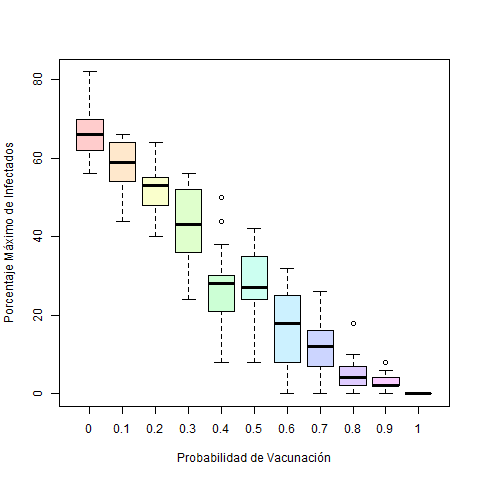
\includegraphics[width=13cm]{BuenaR1.png}
\end{center}
\caption{Cambio en el porcentaje m\'aximo de infectados con respecto  a la probabilidad de generar agentes vacunados en un modelo de punto intermedio aleatorio}
        \label{f3}
\end{figure}

Analizando la figura \ref{f3} se concluye en el reto uno, que la variedad que el modelo de punto intermedio aleatorio aporta al sistema multiagente es notoria. A diferencia del sistema con trayectorias fijas, en este los agentes alcanzan m\'as sitios del \'area a su vez que se cruzan con m\'as agentes y esto aumenta la probabilidad de que los agentes en estado infectado propaguen. Con este nuevo patr\'on de movimiento el porcentaje de infectados ha aumentado en cada una de sus variaciones de probabilidades, a excepci\'on del caso aislado de probabilidad uno.


  \bibliography{P6}
  \bibliographystyle{plainnat}
\end{document}